\documentclass[11pt,a4paper]{ctexart}

\usepackage{amsmath,amssymb,bm}
\usepackage{geometry}
\usepackage{enumitem}
\usepackage{fancyhdr}
\usepackage{lastpage}
\usepackage{xcolor}
\usepackage{tcolorbox}
\usepackage{tikz}
\usepackage{titlesec}
\usepackage{microtype}
\usetikzlibrary{arrows.meta,calc}

\geometry{left=2.15cm,right=2.15cm,top=2.0cm,bottom=2.0cm}
\setlength{\parindent}{2em}
\setlength{\parskip}{0.25em}
\linespread{1.12}

\definecolor{mainblue}{RGB}{39,91,150}
\definecolor{lightblue}{RGB}{232,241,252}
\definecolor{darkgray}{RGB}{65,65,65}
\definecolor{lightgray}{RGB}{245,246,248}

\titleformat{\section}{\large\bfseries\color{mainblue}}{}{0em}{}[\titlerule]
\titleformat{\subsection}{\normalsize\bfseries\color{darkgray}}{}{0em}{}
\titlespacing*{\section}{0pt}{0.9em}{0.45em}
\titlespacing*{\subsection}{0pt}{0.65em}{0.25em}

\setlist[enumerate]{leftmargin=2.2em,itemsep=0.25em,topsep=0.25em}
\setlist[itemize]{leftmargin=2.0em,itemsep=0.2em,topsep=0.2em}

\pagestyle{fancy}
\fancyhf{}
\lhead{\small 格物助航｜每日一练}
\rhead{\small 2026.6.7}
\cfoot{\small 第 \thepage\ 页 / 共 \pageref{LastPage} 页}
\renewcommand{\headrulewidth}{0.4pt}

\newtcolorbox{problemBox}{
  colback=lightblue,
  colframe=mainblue,
  arc=2mm,
  boxrule=0.7pt,
  left=1.0em,
  right=1.0em,
  top=0.8em,
  bottom=0.8em,
  before skip=0.6em,
  after skip=0.8em
}

\newtcolorbox{tipBox}{
  colback=lightgray,
  colframe=darkgray,
  arc=1.5mm,
  boxrule=0.5pt,
  left=0.9em,
  right=0.9em,
  top=0.6em,
  bottom=0.6em,
  before skip=0.5em,
  after skip=0.5em
}

\newcommand{\dd}{\mathrm{d}}
\newcommand{\ii}{\bm{i}}
\newcommand{\jj}{\bm{j}}

\begin{document}

\begin{center}
  {\Large\bfseries\color{mainblue} 格物助航｜每日一练}\par
  \vspace{0.25em}
  {\large 力学第二章：牛顿力学的基本定律}\par
  \vspace{0.35em}
  {\small 2026年6月7日}\par
  \vspace{0.35em}
  {\small 编写：谢奕明}
\end{center}

\vspace{-0.3em}

\section*{解题技巧和思路}
\begin{tipBox}
在惯性系内求解动力学问题时，大致需要如下步骤：
\begin{enumerate}
\item \textit{写出所选取的参考系，给出建立的坐标系，注意正方向的选取；}
\item \textit{确定受力分析的研究对象，找出所受外力（真实力），根据需要在给定坐标系下写出其矢量形式；}
\item \textit{给出约束条件；}
\item \textit{列出动力学方程（注意检查未知数的数量和方程的个数）；}
\item \textit{将动力学方程和约束方程联立，解出未知的力学量。}
\end{enumerate}
\end{tipBox}
\section*{习题再现}
\begin{problemBox}
\noindent\textbf{题目}\quad
质量为$M$的斜面体置于光滑水平面，斜面倾角为$\alpha$，质量$m$的小物块放在斜面上，各接触面光滑。求：

（1）不施加水平恒力$F$时，$m$、$M$各自相对地面的加速度；

（2）若要$m$与$M$保持相对静止，需要对斜面施加多大的水平恒力$F$。

\vspace{0.6em}
\begin{center}
\includegraphics[width=0.62\textwidth]{fig_6.7/fig_1.png}
\end{center}
\end{problemBox}

\section*{详细解法}

\subsection*{第一问的求解}
选取地面为惯性参考系，建立直角坐标系如图，$x$轴水平向右为正，$y$轴竖直向上为正。分开对物块和斜面受力分析。不施加水平恒力$F$时，两物体的受力分析如下图所示：
\vspace{0.4em}
\begin{center}
\includegraphics[width=0.92\textwidth]{fig_6.7/fig_2.png}
\end{center}
\vspace{0.4em}

设斜面$M$的加速度为$a_M$，两分量为$a_{Mx}$和$a_{My}$；设小物块$m$的加速度为$a_m$，分量为$a_{mx}$和$a_{my}$。由于斜面只能在地面上滑动，所以$ a_{Mx} = a_M$，$a_{My} = 0$

由于物块$m$始终沿斜面运动，因此$m$相对于$M$的加速度方向与斜面平行。相对加速度$\boldsymbol{a}_{m,M}=\boldsymbol{a}_m-\boldsymbol{a}_M$的两分量分别等于$a_{mx}-a_M$和$a_{my}$，其斜率满足斜面倾角关系：
\[
\frac{a_{my}}{a_{mx}-a_M} = \tan\alpha
\]
即
\[
a_{my} = (a_{mx}-a_M)\tan\alpha \tag{1}
\]

对斜面$M$列牛顿第二定律：
\[
\begin{cases}
N_2 \sin\alpha = M a_M \\
N_1 - Mg - N_2 \cos\alpha = 0
\end{cases} \tag{2}
\]

对小物块$m$列牛顿第二定律：
\[
\begin{cases}
-N_2 \sin\alpha = m a_{mx} \\
N_2 \cos\alpha - mg = m a_{my}
\end{cases} \tag{3}
\]

包括约束方程，我们共得到五个方程，其中有两个力和三个加速度分量待求解，共五个未知数。我们现在可以确定，我们完全可以把本问求解了。接下来的步骤便是数学上的。

联立(2)(3)的第一式得：
\[
 a_{mx} = -\frac{M}{m}a_M \tag{4}
\]

将(4)代入(1)得：
\[
a_{my} = \left(-\frac{M}{m}a_M - a_M\right)\tan\alpha = -\frac{M+m}{m}a_M \tan\alpha \tag{5}
\]

由(2)得$N_2 = \frac{M a_M}{\sin\alpha}$，代入(3)的第二式并结合(5)：
\[
\frac{M a_M}{\sin\alpha}\cdot\cos\alpha - mg = m\cdot\left(-\frac{M+m}{m}a_M \tan\alpha\right)
\]

化简后解得斜面加速度：
\[
\boxed{a_M = \frac{mg \sin\alpha \cos\alpha}{M + m \sin^2\alpha}}
\]

代入(4)(5)得物块$m$的加速度分量：
\[
\boxed{a_{mx} = -\frac{Mg \sin\alpha \cos\alpha}{M + m \sin^2\alpha}, \quad a_{my} = -\frac{(M + m)g \sin^2\alpha}{M + m \sin^2\alpha}}
\]
符号表示方向，遵循我们规定的坐标系。

\subsection*{第二问的求解}
选取加速运动的斜劈$M$为非惯性参考系，建立随斜劈平动的直角坐标系$Ox'y'$，$x'$轴水平向右为正，$y'$轴竖直向上为正。施加水平恒力$F$后，两物体相对静止，受力分析如下图所示：
\vspace{0.4em}
\begin{center}
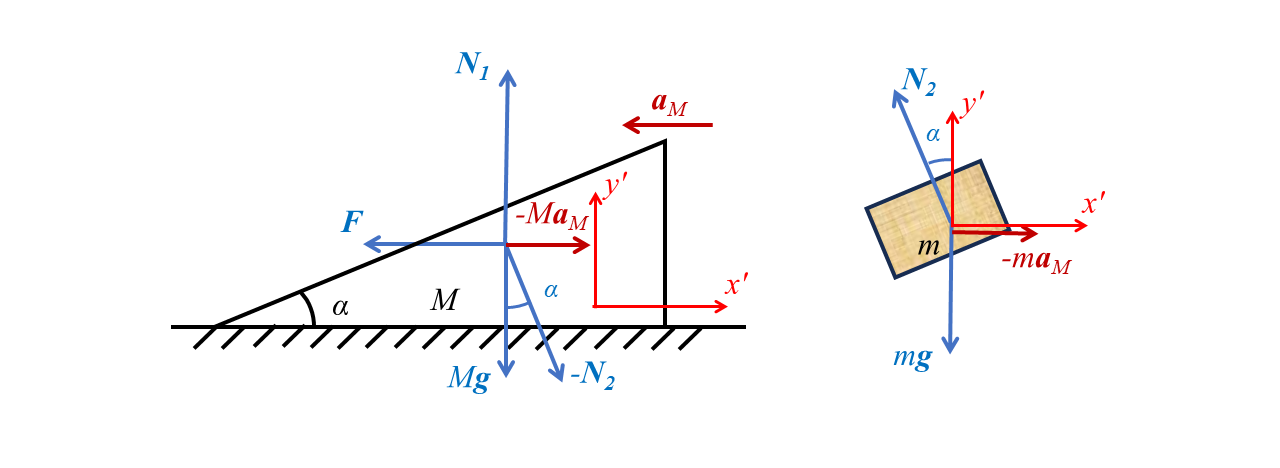
\includegraphics[width=0.92\textwidth]{fig_6.7/fig_3.png}
\end{center}
\vspace{0.4em}

设斜劈相对地面的加速度为$a_M$。在非惯性系中，小物块受到惯性力$-m\boldsymbol{a}_M$，斜面受到惯性力$-M \boldsymbol{a}_M$，方向与$a_M$相反，如图所示。

依照题意，在所选取的参考系内，斜面和小物块均静止，小物块平衡方程为：
\[
\begin{cases}
-N_2\sin\alpha - ma_M = 0 \\
N_2\cos\alpha - mg = 0
\end{cases} \tag{6}
\]
斜面的平衡方程：
\[
\begin{cases}
N_2 \sin\alpha - F - M a_M = 0 \\
N_1 - Mg - N_2 \cos\alpha = 0
\end{cases} \tag{7}
\]

有三个力和一个加速度为未知数，所以共四个未知数；已列出共四个方程，本问题可以求解。
消元最终得所需水平恒力：
\[
\boxed{F = (M+m)g\tan\alpha}
\]
方向水平向左，与图示一致。

\section*{技巧与知识点}
\begin{tipBox}
\begin{enumerate}
  \item \textbf{惯性系解题思路：}如果选取的参考系为惯性系，切勿引入惯性力，注意找全所有力，联立牛顿方程求解。
  \item \textbf{非惯性系使用规则：}在加速斜劈参考系分析时，必须额外添加惯性力，此时所列的动力学方程必须是在非惯性系内的，注意不要把相对地面的加速度当成非惯性系内的加速度。
  \item \textbf{加速度约束关键：}两物体相对滑动时，相对速度、相对加速度沿斜面（很多人会认为是相对地面的速度、加速度沿斜面，最终将会导致结果错误），此时把相对速度、相对加速度水平分量和竖直分量写出后用几何关系约束往往能避免出错。
  \item \textbf{未知数与方程校验：}列式完毕后统计未知量与独立方程数量，提前判断方程组可解性。
  \item \textbf{符号规范：}全程按照预先设定的坐标系正方向写出矢量分量，由计算结果正负判断矢量实际方向（最终结果出现负号意味着实际方向是我们假设方向的反方向，但模长是对的），避免全都用绝对值导致矢量加减时搞错大小和方向。
\end{enumerate}
\end{tipBox}

\section*{复习建议}
牛顿定律板块解题流程总结：
\[
\text{选定参考系与坐标系}
\longrightarrow
\text{受力分析}
\longrightarrow
\text{给出约束方程和动力学方程}
\longrightarrow
\text{联立求解未知量}.
\]
建议复习做题时重点关注：
\begin{enumerate}
  \item 思考选取谁为研究对象受力分析、选取何种参考系和坐标系，以追求减少未知数，实现简化求解；
  \item 光滑或粗糙接触面的斜面问题，注意哪些面涉及摩擦力，避免漏掉摩擦力；
  \item 注意观察约束的形式，利用恰当方法给出正确的约束方程。
\end{enumerate}

\end{document}